\section{Methodology}

    Previous work on synthesizing fine grained concurrent programs assumed infinte resources (hardware accelerators).
    In practice this is not true. 
    One straightforward direction is to consider a more global scheduling approach to reuse resources.
    However, coming up with a sound global analysis that respects all consistency rules of the concurrency model might be non-trivial task.
    Instead, I propose to address the resource constraint problem by performing an optimization that merges two or more threads.
    Previous work has shown that optimizations do significantly improve the resource requirements. 
    However, the optimizations considered were only for sequential programs; while merging two threads is something for concurrent programs. 
    Hence, we investigate whether this optimization indeed helps our case.

    The main goal is to identify if we can minimize resource utilization while performing synthesis of concurrent programs such as above.
    We assume from previous work that synthesis is done per-thread; each thread is scheduled independently and allocated its own share of resources.
    In this endeavor, I have only addressed the correct scheduling and performing this optimization at the pre-scheduling stage.
    I do not implement the full HLS process; the program; if concurrent, cannot be synthesized into VHDL as of now. 

    %Explain here what you exactly need 
    \subsection{Concurrency Model}

        There are several shared memory concurrency models that exist to date.
        Previous work has mainly focused on C based concurrency.
        The C concurrency model semantics is fairly non-trivial to tackle as well as implement. 
        Hence, I choose a standard intuitive model widely understood; Sequential Consistency\cite{Lamport79}. 

    \subsection{Types of Programs}

        The programs are considered to be a set of statements of the following format 
        \begin{align}
            a \ = \ b \ + \ cs
        \end{align}
        Here $a$ refers to some memory.
        $b$ and $cs$ can be either memory or constants. 

        Memory can be termed as local ($a$ and $b$) or global/shared ($cs$ - any memory name ending with $s$).

        Each program is viewed as a set of threads; each of which have the following statements as above. 
        There are no coniditional branching statements, nor loops. 
        
    \subsection{Code Base Utilized}

        For the implementation, I reuse the existing code base from Assignment. 
        The assignment dealt only with sequenital programs of the above form. 
        The extension thus, must be done to incorporate concurrency reflecting SC.

    \subsection{Additions to Code base}
    
        \paragraph*{Threads}
            The notion of threads is easily captured by the code-base by representing each thread as its own DFG. 
            
        \paragraph*{Correct Scheduling}

            One important thing to address is that of ensuring correct scheduling in a concurrent context.
            \cite{DBLP:conf/fpga/RamanathanFWC17} showed that without adding extra memory dependencies, one can get an incorrect schedule for synthesis. 
            Thus, the solution was to add additional dependencies between memory accesses which are shared. 
            For sequential consistency, the dependencies were identified to be between every shared memory access in the same thread.
            Fig~\ref{scord} represents the following functions that were created for this
            \begin{figure}
                \centering
                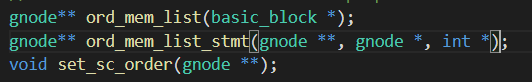
\includegraphics[scale=0.5]{Sc-order.PNG}
                \caption{Three functions created to take a thread and add additional memory dependencies respecting Sequential Consistency.}
                \label{scord}
            \end{figure}

            Adding these dependency edges, the scheduler must also incorporate this information while alloting an action to a specific clock cycle time stamp. 
            Fig~\ref{Schd} showcases the code snippet that was added for this. 
            Note that because we still use the previous approach of independently scheduling each thread, these changes were identified to be sufficient for correct scheduling. 
            \begin{figure}
                \centering
                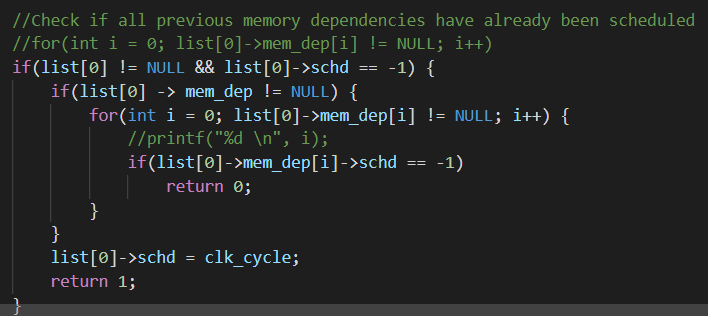
\includegraphics[scale=0.5]{Schd.PNG}
                \caption{Code snippet added to factor in memory dependencies while scheduling}
                \label{Schd}
            \end{figure}

        \paragraph*{Merging Optimization}
    
        I have implemented a DFG as a set of DFGs in my code base.
        Thus, merging was equivalent to simply adding one DFG into another. 
        While merging, memory dependencies that are newly introduced must also be taken care of.
        This differentiates the different merging combinations.
        Since the DFG set is implemented as an array of DFGs, the implicit array order was used to retain the memory order after merging.
 
        Fig~\ref{merge} represents the above idea. 
        Here $t1$ and $t2$ are two threads which are a set of DFGs. 
        $merge$ is the new program that is to be constructed using the elements of $t1$ and $t2$. 
        \begin{figure}
            \centering
            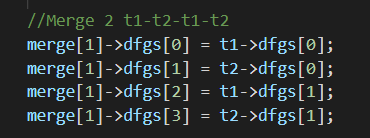
\includegraphics[scale=0.5]{Merge.PNG}
            \caption{Merging is equivalent to just adding and mixing DFG components of one thread with another}
            \label{merge}
        \end{figure}

        %Insert code snippet

    \paragraph*{Soundness?}

        An important factor to consider is whether such merging is a sound Transformation. 
        \cite{DBLP:journals/pcs/MoiseenkoPK21}, in their survey paper, do however, mention merging as a sound transformation under Sequential Consistency (SC).
        So a formal proof is not required.
 
    %Explain how you combine all of them into one specific total order on memory events

    %Show code snippets that you inserted for them in your existed code base

    %Showcase why this works (sketch proof?)